% 若编译失败,且生成 .synctex(busy) 辅助文件,可能有两个原因:
% 1. 需要插入的图片不存在:Ctrl + F 搜索 'figure' 将这些代码注释/删除掉即可
% 2. 路径/文件名含中文或空格:更改路径/文件名即可

% --------------------- 文章宏包及相关设置 --------------------- %
% >> ------------------ 文章宏包及相关设置 ------------------ << %
% 设定文章类型与编码格式
\documentclass[UTF8]{article}		
\input{../.config/config_for_NonlinearCircuitExperiment.tex}



%%%%%%%%%%%%%%%%%%%%%%%%%%%%%%%%%%%%%%%%%%%%%%%%%%%%%%%%%%%%%%%%
% 仅需修改页眉、实验名称、实验日期
%%%%%%%%%%%%%%%%%%%%%%%%%%%%%%%%%%%%%%%%%%%%%%%%%%%%%%%%%%%%%%%%


%%%%%%%%%%%%%%%%%% 1. 修改页眉内容 %%%%%%%%%%%%%%%%%%
\rhead{NCE-06 Multiplier-Based Mixer (2025.12.04, 丁毅)}

% 开始编辑文章
\begin{document}
\begin{center}\large
    \vspace*{-0.8cm}
    \noindent{\huge\bfseries《\ \ 非\ \ 线\ \ 性\ \ 电\ \ 路\ \ 实\ \ 验\ \ \ 》\ \ 实\ \ 验\ \ 报\ \ 告 }
    \\\vspace{0.1cm}
    \noindent{ 
    {\bfseries 
%
%%%%%%%%%%%%%%%%%% 2. 修改实验名称 %%%%%%%%%%%%%%%%%%
    实验名称:\uline{\hspace{0.8cm} Multiplier-Based Mixer \hspace{0.8cm}}
%
    }\hspace{0.4cm}
    指导教师:\uline{\hspace{0.5cm}冯鹏\ \ fengpeng06@semi.ac.cn     \hspace{0.5cm}}
    }
    \\\vspace{0.1cm}
    \noindent
    {
    姓名:\uline{\,\,\,丁毅\,\,\,}\hspace{0.2cm}
    学号:\uline{\,\,\,{ 2023K8009908031}\,\,\,}\hspace{0.2cm}
    班级/专业:\uline{\,\,\,{2308/电子信息}\,\,\,}\hspace{0.2cm}
    分组序号:\uline{\,\,\,{2-06}\,\,\,}
    }
    \\\vspace{0.1cm}
    \noindent{
%
%%%%%%%%%%%%%%%%%% 3. 修改实验日期 %%%%%%%%%%%%%%%%%%
    实验日期:\uline{\,\,{2025.12.04}\,\,}\hspace{0.2cm}
%
    实验地点:\uline{\,\,\,西实验楼 (8 号楼) { 308}\,\,\,}\hspace{0.2cm}
    是否调课/补课:\uline{\hspace{0.1cm}否 \hspace{0.1cm}}\hspace{0.2cm}
    成绩:\uline{\hspace{0.6cm}}
    }
\end{center}
\vspace{-0.4cm}
\noindent\rule{\textwidth}{0.075em}   % 分割线
\vspace{-1.0cm}


% 生成目录
\setcounter{tocdepth}{3}  % 目录深度为 2(不显示 subsubsection)
\noindent\tableofcontents\thispagestyle{fancy}   % 显示页码、页眉等
%\newpage
\vspace{0.5cm}
\noindent\rule{\textwidth}{0.075em}   % 分割线

% ------------------------ 文章信息区 ------------------------ %
% ------------------------ 文章信息区 ------------------------ %



%%%%%%%%%%%%%%%%%%%%%%%%%%%%%%%%%%%%%%%%%%%%%%%%%%%%%%%%%%%%%%%%%%%%%%%%%%%%%%%%%
%%%%%%%%%%%%%%%%%%%%%%%%%%%%%%%%% 下面是正文内容 %%%%%%%%%%%%%%%%%%%%%%%%%%%%%%%%%
%%%%%%%%%%%%%%%%%%%%%%%%%%%%%%%%%%%%%%%%%%%%%%%%%%%%%%%%%%%%%%%%%%%%%%%%%%%%%%%%%

\section{实验目的}

\begin{enumerate}
\item 学习并掌握变频电路的相关理论;
\item 掌握乘法混频电路的工作原理和调试方法。
\end{enumerate}



\section{实验仪器}

\begin{enumerate}
\item 高频实验箱 - 乘法调幅/混频实验板 (031132201809392)
\item 示波器 RIGOL MSO2202A  (080103201901376)
\item 信号发生器 GWINSTEK AFG-2225  (080102201901355)
\item 万用表 LINIT- UT61A (C181503983)
\end{enumerate}



\section{实验原理}

\subsection{混频器基本原理}

在通信系统中,经常需要将信号自某一频率变换为另一频率,例如把
一个已调的高频信号变成另一个较低频率的同类已调信号 (Downconversion, 下变频),又或者把一个已调的低频信号变成另一个较高频率的同类已调信号 (Upconversion, 上变频)。完成这种频率变换的电路称为变频器或混频器,它是无线通信系统中的重要组成部分。

混频器 (Mixer) 通常由非线性器件作为核心 (二极管、晶体管、模拟乘法器模块),配合其它有源模块和无源器件组成,这些器件会将输入信号注入到非线性器件中,由其完成混频操作。近年混频器方面的技术前沿表明,混频器的带宽主要受到无源器件限制,而非受到二极管或晶体管的限制,因为后者的带宽一般能很好地满足要求。因此,设计高性能混频器的关键在于合理设计无源器件网络,以实现所需的频率响应特性。

作为射频系统中的关键组件,混频器的主要参数有:

\begin{enumerate}
\item 功率增益 (Power Gain):$G_{p} = \frac{P_{out}}{P_{in}}$,表示输出信号功率与输入信号功率之比;
\item 噪声系数 (Noise Figure):$NF = \frac{SNR_{in}}{SNR_{out}}$,表示输入信号与输出信号的信噪比之比;
\item 混频失真与干扰:混频器的失真包括频率失真等非线性失真,此外由于器件的非线
性还存在着组合频率干扰,这些干扰往往伴随有用信号而存在,严重影响混频器正常工
作,因此需关注减小混频失真与干扰;
\item 选择性:指混频器选出有用输出信号而滤除其他干扰信号的能力,选择性越好输出的频谱纯度越高,往往取决于输出端的带通滤波器的性能。
\end{enumerate}

\subsection{实验电路简要分析}

本次实验采用的 Multiplier-Based Mixer (乘法器混频器) 如 Figure \ref{fig__multiplier_based_mixer} 所示,用于将高频输入信号 $f_{in}$ 下变频 (Downconversion) 为中频输出信号 $f_{out}$。

该电路整体上也分为两级,对混频功能而言,第一级为由模拟乘法器构成的混频电
路,配合外围的电容电阻来控制输入信号的幅度;频率为 455 kHz 的输出经电容耦合接入作为输出隔离的第二级 (Common Collector)。


\begin{figure}[H]\centering
    \includegraphics[width=\columnwidth]{assets/circuit.png}
    \caption{Multiplier-Based Mixer Schematic}
    \label{fig__multiplier_based_mixer}
\end{figure}




实验时,将跳线 J1, J2, J3 的二号端口连接到一号端口 (也即“混频”功能,连接到三号端口对应“调幅”功能),并在 IN1 (TP1) 和 IN3 (TP3) 分别输入本振 $f_{in} = 10.245 \mathrm{MHz}$ 和载波 $f_c = 10.700 \ \mathrm{MHz}$,此时混频器输出中频信号 $f_{out} = |f_{in} - f_c| = 455 \mathrm{kHz}$。

\section{实验内容与步骤}






\begin{enumerate}
\item 在实验箱上插上集成乘法器混频电路实验模块和正弦波振荡电路实验模块,接
通实验箱电源。
\item 在 IN1 端接入由信号发生器产生的 10.245 MHz 本振信号;然后利用 NCE-05 实验中的正弦波振荡电路输出 10.7 MHz 载波信号,接入混频器模块 IN3 (TP3) 端;
\item 调节 IN1 输入信号幅度和电阻 W1,用示波器采样输出波形,将数据导出到电脑用 MATLAB 进行傅里叶分析,直至得到 455 kHz 输出信号;
\item 调节可变电阻 W2,继续用 MATLAB 对输出信号进行傅里叶分析,直至得到幅度合适、信噪比最好、失真度最小的 455 kHz 输出信号;
\end{enumerate}

\section{实验结果与分析}

设置输入本振频率为 $f_{in} = 10.245 \ \mathrm{MHz}$,载波频率为 $f_c = 10.700 \ \mathrm{MHz}$,用示波器测量得到本振信号 $f_{in}$ 和下变频后的输出信号 $f_{out}$ 如 Figure \ref{fig__measured_waveforms} 所示。


\begin{figure}[H]\centering
    \includegraphics[width=\columnwidth]{NCE-06 Multiplier-Based Mixer/assets/CH1 本振 (10.245 MHz) 与 CH2 下变频输出 (0.455 MHz).png}
    \caption{Measured waveforms of input signal (CH1, blue, 10.245 MHz) and down-converted output (CH2, red, 0.455 MHz)}
    \label{fig__measured_waveforms}
\end{figure}


为对比输入输出信号的频谱特性,分别对输入本振信号和输出中频信号进行傅里叶变换分析,结果如 Figure \ref{fig__spectrum_input} 至 Figure \ref{fig__spectrum_comparison} 所示。注意实验中使用的是低本振信号 ($f_{in} < f_c$),因此其频率偏移量应取反,也即:
\begin{gather}
\text{for $f_{in}$:\ \ }
f_{m} = -(f - f_{in}),\quad \text{for $f_{out}$:\ \ } f_{m} = f - f_{out}
\\ 
\text{where\ $f_m$ denotes\ the\ offset\ frequency.}
\end{gather}


\newpage
\begin{figure}[H]\centering
    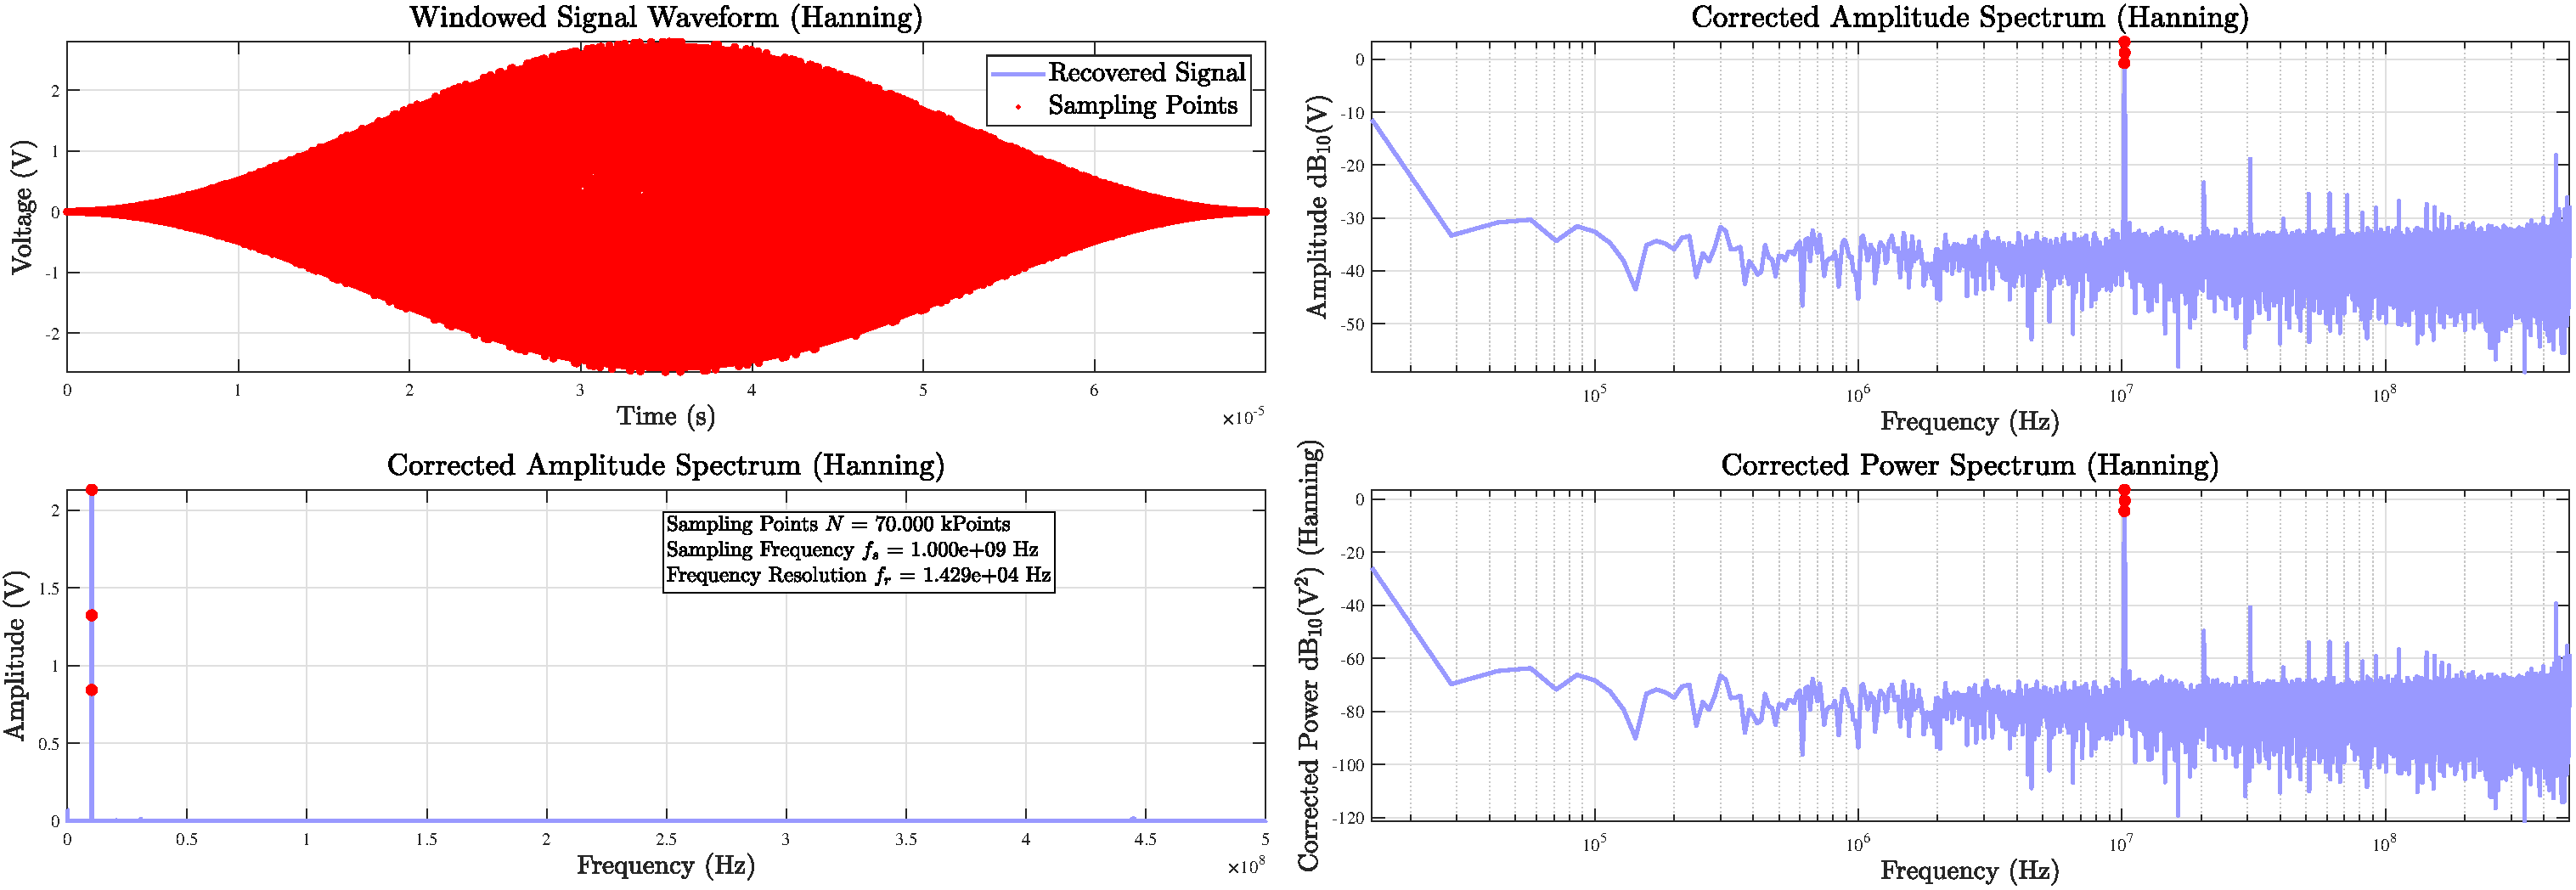
\includegraphics[width=\columnwidth]{NCE-06 Multiplier-Based Mixer/assets/spectrum_in.pdf}
    \caption{Spectrum analysis of input signal (10.245 MHz)}
    \label{fig__spectrum_input}
\end{figure}

\begin{figure}[H]\centering
    \includegraphics[width=\columnwidth]{NCE-06 Multiplier-Based Mixer/assets/spectrum_out.pdf}
    \caption{Spectrum analysis of down-converted output signal (0.455 MHz)}
    \label{fig__spectrum_output}
\end{figure}

\begin{figure}[H]\centering
    \includegraphics[width=\columnwidth]{NCE-06 Multiplier-Based Mixer/assets/spectrum_in_out.pdf}
    \caption{Spectrum comparison between input signal (10.245 MHz) and down-converted output signal (0.455 MHz)}
    \label{fig__spectrum_comparison}
\end{figure}

从 Figure \ref{fig__spectrum_comparison} 可见,输入信号和输出信号的频谱特性 (形状等、变化趋势等) 基本一致,在频率偏移范围 $f_m \in (-0.10 \ \mathrm{MHz},\ \ 0.10\ \mathrm{MHz})$ 内,可近似认为 \textbf{“除了约 12.5 dB 的功率衰减外,二者频谱基本相同”},说明乘法混频器实现了预期下变频功能。




\section{思考题}

\subsection{改变信号发生器提供的 IN1 输入频率时,输出波形和频率作何变化,为什么?}

保持其它参数不变,改变本振输入信号的频率 $f_{in}$,得到带有不同幅度的输出频率 $f_{out} = 10.7 \ \mathrm{MHz} - f_{in}$,如下图所示:


\begin{figure}[H]\centering
    \includegraphics[width=0.95\columnwidth]{NCE-06 Multiplier-Based Mixer/assets/CH1 本振 (10.240 MHz) 与 CH2 下变频输出 (0.455 MHz).png}
    \caption{Measured waveforms of input signal (CH1, blue, 10.240 MHz) and down-converted output (CH2, red, 0.460 MHz)}
    \label{fig__measured_waveforms_variant1}
\end{figure}

\begin{figure}[H]\centering
    \includegraphics[width=0.95\columnwidth]{NCE-06 Multiplier-Based Mixer/assets/CH1 本振 (10.230 MHz) 与 CH2 下变频输出 (0.455 MHz).png}
    \caption{Measured waveforms of input signal (CH1, blue, 10.230 MHz) and down-converted output (CH2, red, 0.470 MHz)}
    \label{fig__measured_waveforms_variant2}
\end{figure}

\begin{figure}[H]\centering
    \includegraphics[width=0.95\columnwidth]{NCE-06 Multiplier-Based Mixer/assets/CH1 本振 (10.200 MHz) 与 CH2 下变频输出 (0.455 MHz).png}
    \caption{Measured waveforms of input signal (CH1, blue, 10.200 MHz) and down-converted output (CH2, red, 0.500 MHz)}
    \label{fig__measured_waveforms_variant3}
\end{figure}

幅度之所以发生改变,是因为混频器输出信号经过了一个带通滤波器,输出信号频率越接近该滤波器的中心频率,衰减量就越小,输出幅值就越大;反之,幅值会越来越小。上图还能观察出,实验板模块上带通滤波器的中心频率并不是 0.455 MHz,而是约为 0.460 MHz。


\newpage
\section*{附录 A\hspace*{20pt} 原始数据记录表}
\addcontentsline{toc}{section}{附录 A\hspace*{6pt} 原始数据记录表} 
\thispagestyle{fancy} 
\noindent \begin{graybox}
注:本次实验所有数据均以 .txt 格式保存在电脑中,已由赵嘉明助教核验过。由于数据基本都为波形采样数据,整体数据量较多,故此处不再单独附上原始数据。
\end{graybox}


\vspace*{\fill}
\begin{center}\Huge{\bfseries 
    附录 B\hspace*{20pt} 实验预习报告
}\end{center}\addcontentsline{toc}{section}{附录 B\hspace*{6pt} 实验预习报告} 
\vspace*{\fill}
\thispagestyle{fancy} 
\includepdf[pages={-}]{NCE-06 Multiplier-Based Mixer/preview/NCE-06 (preview report).pdf}


% 附录
\section*{附录 C \hspace*{20pt} MATLAB Codes}
\addcontentsline{toc}{section}{附录 C \hspace*{6pt} MATLAB Codes} 
\thispagestyle{fancy} 
\lstinputlisting{d:/a_RemoteRepo/GH.MatlabCodes/本科课程代码/Non-Linear Circuits/NCE_06.m}

































\end{document}

% VScode 常用快捷键:

% F2:                       变量重命名
% Ctrl + Enter:             行中换行
% Alt + up/down:            上下移行
% 鼠标中键 + 移动:           快速多光标
% Shift + Alt + up/down:    上下复制
% Ctrl + left/right:        左右跳单词
% Ctrl + Backspace/Delete:  左右删单词    
% Shift + Delete:           删除此行
% Ctrl + J:                 打开 VScode 下栏(输出栏)
% Ctrl + B:                 打开 VScode 左栏(目录栏)
% Ctrl + `:                 打开 VScode 终端栏
% Ctrl + 0:                 定位文件
% Ctrl + Tab:               切换已打开的文件(切标签)
% Ctrl + Shift + P:         打开全局命令(设置)

% Latex 常用快捷键:

% Ctrl + Alt + J:           由代码定位到PDF


